\documentclass[12pt]{article}
\usepackage[margin=1in]{geometry}
\usepackage{graphicx,booktabs,url,setspace,caption,amsmath,float}
\usepackage[T1]{fontenc}\usepackage{lmodern}\usepackage[hidelinks]{hyperref}\usepackage{xurl}
\captionsetup{font=small,labelfont=bf,justification=justified}
\setstretch{1.15}
\title{Food Environment and Adult Diabetes Prevalence Across U.S. Counties: An Ecological Analysis Accounting for Socioeconomic Factors and Physical Inactivity}
\author{Haoxi Hu\thanks{Corresponding author: \href{mailto:hu.haoxi@northeastern.edu}{hu.haoxi@northeastern.edu}}\\[2pt]
\small Khoury College of Computer Sciences and Bouv\'e College of Health Sciences,\\
\small Northeastern University}
\date{}
\begin{document}
\maketitle
\vspace{-2em}
\begin{abstract}
Background: Counties with a poorer food environment may have higher rates of diabetes, but income, insurance, rurality, and physical inactivity travel with food access and could account for the pattern. Methods: This cross-sectional, ecological study used the 2025 County Health Rankings \& Roadmaps data for 3,100 U.S. counties. The Food Environment Index (a 0 to 10 score, higher is better) was compared with age-adjusted adult diabetes prevalence using Spearman rank correlation and ordinary least squares regression with heteroskedasticity-robust standard errors, adjusting for median household income, percent uninsured, percent rural, and physical inactivity. Obesity was left out of the main model because it may lie on the path between food environment and diabetes, and was added in a sensitivity analysis. Results: A better Food Environment Index was strongly associated with lower diabetes prevalence before adjustment (Spearman $\rho = -0.63$; unadjusted $R^2$ = 0.37). After adjustment the association was much smaller but still present: each 1-point higher index was associated with 0.23 percentage points lower prevalence (95\% CI -0.28 to -0.19; standardized coefficient -0.12). The full model explained 0.81 of the variation in county diabetes prevalence, but the food environment added only 0.8 percentage points of that, and physical inactivity dominated (standardized coefficient 0.82). Results were similar across six sensitivity analyses. Conclusions: A poorer food environment is associated with higher county diabetes prevalence after accounting for income, insurance, rurality, and inactivity, but the independent association is small. These ecological, cross-sectional results cannot show that food environments affect diabetes in individuals.
\end{abstract}
\noindent\textbf{Keywords:} food environment; diabetes; county health; socioeconomic factors; ecological study

\section*{Introduction}
Diabetes is not spread evenly across places, and county prevalence differs widely. Reviews describe a robust link between neighborhood socioeconomic disadvantage and diabetes (Bilal et al., 2018), and the broader literature treats social determinants of health as central to how diabetes develops (Hill-Briggs et al., 2021). Public health researchers have long asked whether features of the neighborhood itself, beyond the characteristics of the people who live there, contribute to this pattern.

One feature of interest is the food environment: how easily residents can reach affordable, healthy food. Researchers have developed several ways to measure food access and to define so-called food deserts, areas where people have limited access to nutritious food (Ver Ploeg et al., 2015). Evidence linking the food environment to diabetes exists but is mixed. In a U.S. cohort followed over time, higher neighborhood exposure to healthy food was associated with a lower risk of developing type 2 diabetes (hazard ratio 0.88, 95\% CI 0.79 to 0.98; Christine et al., 2015), while a review concluded that some findings on food environments and diabetes risk conflict (Bilal et al., 2018). The same review described the link between neighborhood socioeconomic status and diabetes as robust and repeatedly replicated, which raises a measurement problem: because food access, income, and insurance coverage are tangled together at the county level, an apparent food environment association may partly reflect these other factors.

This study asks a focused question: is a poorer county food environment associated with higher adult diabetes prevalence after accounting for socioeconomic and behavioral factors that are not themselves downstream of the food environment? We use the Food Environment Index from County Health Rankings \& Roadmaps, a county-level composite score, together with county estimates of diabetes prevalence. We adjust for median household income, the share of residents without health insurance, the share living in rural areas, and physical inactivity. We deliberately do not adjust for adult obesity in the main model. Obesity may be one of the ways a food environment relates to diabetes, so adjusting for it could hide part of the association we want to measure; we examine it separately as a sensitivity check. We report the size of the association, not only whether it is statistically distinguishable from zero, and we compare it with the other factors in the model.

\section*{Methods}
\subsection*{Study design and data sources}
This was a cross-sectional ecological study, meaning the unit of analysis is the county and all variables describe counties, not individuals. We used the County Health Rankings \& Roadmaps 2025 Annual Data Release analytic file (University of Wisconsin Population Health Institute, 2025), which assembles county measures from national sources (Remington et al., 2015). The file contained 3,152 county-level rows. We removed state-level summary rows and merged variables on the five-digit county FIPS code (the standard federal county identifier); every row matched (3,152 of 3,152).

The file reports each measure for a specific data year, as documented by County Health Rankings \& Roadmaps. The Food Environment Index combines two indicators, limited access to healthy foods (data year 2019) and food insecurity (2022), each weighted equally. Diabetes prevalence, physical inactivity, and the percent uninsured under age 65 are for 2022. Median household income is for 2023, and percent rural is from the 2020 Census. The outcome, diabetes prevalence, and the physical inactivity measure are model-based county estimates produced from survey data (the Behavioral Risk Factor Surveillance System), not direct counts of every resident. Model-based estimates borrow strength across places to stabilize small areas (Zhang et al., 2014), which means county values partly reflect the model and not only local survey responses.

\subsection*{Variables}
The outcome was age-adjusted prevalence of diagnosed diabetes among adults aged 18 and over (percent). The exposure was the Food Environment Index, scored from 0 (worst) to 10 (best). Covariates were median household income (in thousands of dollars), percent of the population under 65 without health insurance, percent of the population living in a census-defined rural area, and percent of adults reporting no leisure-time physical activity (age-adjusted). Adult obesity prevalence was used only in a sensitivity analysis.

\subsection*{Statistical analysis}
We kept counties with complete data on all six main variables (3,100 of 3,152; the Food Environment Index was missing for 52 counties, including all 17 Connecticut rows (its legacy counties and planning regions have no index values) and 35 counties elsewhere, and each other variable was missing for 8 or 9 counties). Because Connecticut contributes no complete counties, the analysis covers 50 jurisdictions: 49 states and the District of Columbia.

We first described each variable and computed Spearman rank correlations, which measure whether two variables rise and fall together without assuming a straight-line relationship. We then fitted ordinary least squares (OLS) regression of diabetes prevalence on the Food Environment Index, first alone and then with income, percent uninsured, percent rural, and physical inactivity. Standard errors were heteroskedasticity-robust (HC3), which keeps confidence intervals valid when the spread of the errors differs across counties. We report coefficients in the original units (percentage points of diabetes prevalence per one-unit change) and standardized coefficients (standard deviations of diabetes prevalence per standard deviation of the predictor), which allow predictors measured on different scales to be compared. We report $R^2$, the share of variation in diabetes prevalence explained by the model, and the increase in $R^2$ attributable to the Food Environment Index.

Model checks included variance inflation factors (VIF; values near 1 indicate little overlap among predictors, and values above 5 to 10 are usually considered a concern), the Breusch-Pagan test for unequal error spread, residual skewness and kurtosis, and Cook's distance, which flags counties with outsized influence. As a descriptive complement, we divided counties into quintiles (five equal-sized groups) of the Food Environment Index and compared mean diabetes prevalence across them, both unadjusted and adjusted for the four covariates.

Sensitivity analyses were: (1) standard errors clustered by state, which allows counties in the same state to be correlated; (2) state fixed effects, which compares counties only with other counties in the same state, with state-clustered errors; (3) adding adult obesity; (4) replacing income with its natural logarithm; (5) using the March 2026 supplemental release of County Health Rankings \& Roadmaps, which updated the Food Environment Index, diabetes, inactivity, uninsured, and obesity measures to 2023 data (this release lacks diabetes values for Kentucky and Pennsylvania counties and does not update income or rurality, so it was used as a check and not as the main dataset); and (6) excluding counties with high influence (Cook's distance above 4 divided by the number of counties). Analyses were implemented in Python with NumPy, SciPy, pandas, and Matplotlib. The data are public and aggregated to counties, so no individual-level data were used.

\section*{Results}
\subsection*{Descriptive statistics}
The 3,100 counties had a mean Food Environment Index of 7.5 (standard deviation 1.2; median 7.6) and a mean diabetes prevalence of 11.1\% (standard deviation 2.3; range 6.0\% to 21.5\%). Table 1 shows all variables. The index distribution had a longer tail toward poorer scores (mean below median).

\subsection*{Unadjusted association}
A better Food Environment Index was strongly associated with lower diabetes prevalence (Spearman $\rho = -0.63$, $p<0.001$). Mean diabetes prevalence fell from 13.3\% in the lowest index quintile to 9.2\% in the highest, a difference of 4.0 percentage points (Figure 1A). In an unadjusted regression, each 1-point higher index was associated with 1.17 percentage points lower prevalence (95\% CI -1.25 to -1.09), and the index alone accounted for 0.37 of the variation.

The index was closely related to the other socioeconomic measures: it correlated 0.70 with median household income. Diabetes prevalence correlated most strongly with physical inactivity ($\rho = 0.87$), followed by income ($\rho = -0.65$) and percent uninsured ($\rho = 0.48$). Percent rural had a weak positive correlation ($\rho = 0.10$).

\subsection*{Adjusted association}
After adjustment, the association between the food environment and diabetes shrank by about 80\% but remained statistically distinguishable from zero (Table 2). Each 1-point higher Food Environment Index was associated with 0.23 percentage points lower diabetes prevalence (95\% CI -0.28 to -0.19, $p<0.001$), equal to 0.28 percentage points per standard deviation of the index. The standardized coefficient was -0.12 (95\% CI -0.15 to -0.10), compared with -0.61 before adjustment. The adjusted difference between the lowest and highest index quintiles was 0.50 percentage points (0.33 to 0.67), compared with the unadjusted difference of 4.0.

The model explained 0.81 of the variation in county diabetes prevalence (adjusted $R^2$ = 0.81, N = 3,100). Removing the Food Environment Index lowered $R^2$ only from 0.81 to 0.80, a change of 0.8 percentage points. The strongest predictor by far was physical inactivity (standardized coefficient 0.82, 95\% CI 0.79 to 0.84). Percent uninsured had a small positive association (0.07, 95\% CI 0.06 to 0.09). Percent rural had a negative association (-0.14, 95\% CI -0.16 to -0.12), the opposite direction from its weak positive unadjusted correlation. Median household income showed no clear association once the other variables were included (0.01, 95\% CI -0.02 to 0.04, $p=0.45$).

\subsection*{Model checks and sensitivity analyses}
Predictors were not strongly overlapping (largest VIF 2.49; Food Environment Index VIF 1.91). The Breusch-Pagan test indicated unequal error spread ($p<0.001$), which is why robust standard errors were used. Residuals were mildly right-skewed (skewness 0.44; excess kurtosis 0.70), 0.8\% of counties had standardized residuals beyond 3, and the largest Cook's distance was 0.020, so no single county dominated the fit.

The Food Environment Index association persisted in every sensitivity analysis (Table 3). With state-clustered errors the coefficient was unchanged by construction (-0.23) but its interval widened (95\% CI -0.36 to -0.11). Comparing counties only within the same state, the coefficient was smaller (-0.17, 95\% CI -0.24 to -0.10; standardized -0.09), and the model $R^2$ rose to 0.91. Adding obesity gave a slightly larger food environment coefficient (-0.26, 95\% CI -0.31 to -0.21), with obesity itself positively associated with diabetes (0.07 percentage points per percentage point, 95\% CI 0.06 to 0.08). Using log income, the 2023 supplemental data (2,919 counties; coefficient -0.24, 95\% CI -0.29 to -0.18; Spearman $\rho = -0.64$), and excluding influential counties (2,910 counties) all left the association close to the main estimate. Income had small associations of differing sign across specifications (positive when obesity was added, negative in the 2023 data and with log income), so the near-zero income finding in the main model is not stable.

\begin{table}[H]
\centering\small
\caption{Characteristics of the 3,100 counties in the main analysis. SD = standard deviation; IQR shown as 25th to 75th percentile; pp = percentage points. Source: County Health Rankings \& Roadmaps 2025 Annual Data Release; author analysis.}
\resizebox{\linewidth}{!}{%
\begin{tabular}{lrrrrrr}
\toprule
Variable & $N$ & Mean & SD & Median & 25th--75th & Range \\
\midrule
Food Environment Index (0-10) & 3,100 & 7.5 & 1.2 & 7.6 & 6.8--8.3 & 0.0--10.0 \\
Adult diabetes prevalence (\%) & 3,100 & 11.1 & 2.3 & 10.8 & 9.4--12.5 & 6.0--21.5 \\
Median household income (\$1,000s) & 3,100 & 65.5 & 16.4 & 62.7 & 54.6--73.0 & 28.6--173.7 \\
Uninsured, under 65 (\%) & 3,100 & 10.5 & 4.7 & 9.4 & 6.9--13.2 & 2.1--37.7 \\
Rural population (\%) & 3,100 & 63.9 & 33.6 & 66.4 & 35.5--100.0 & 0.0--100.0 \\
Physical inactivity (\%) & 3,100 & 26.4 & 5.2 & 26.0 & 22.8--29.8 & 11.8--47.3 \\
\bottomrule
\end{tabular}%
}
\end{table}

\begin{figure}[H]
\centering
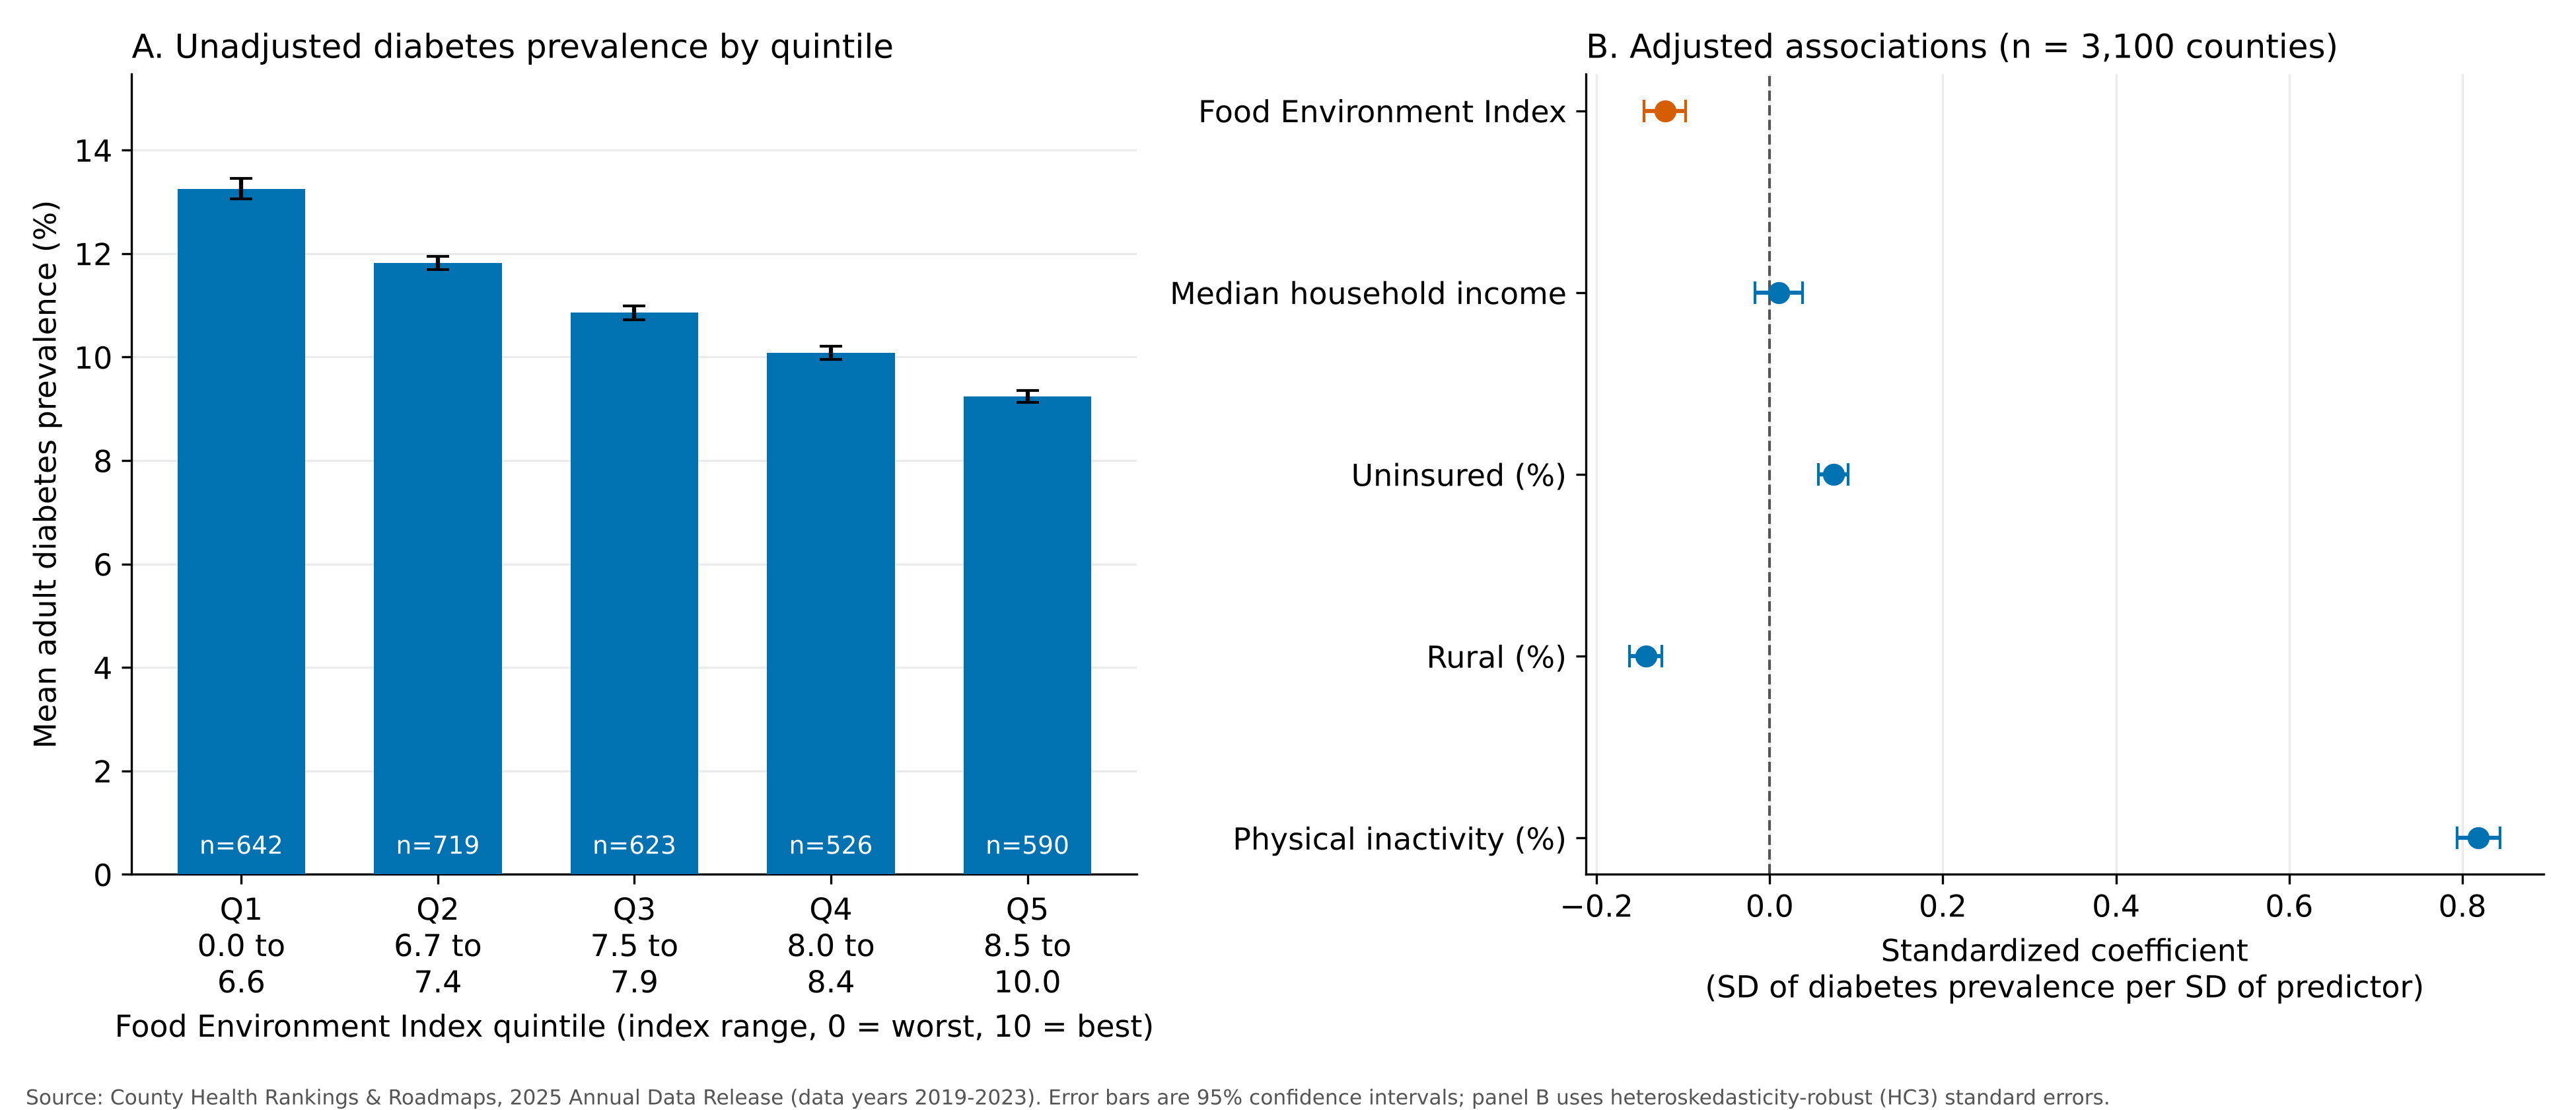
\includegraphics[width=\linewidth]{figures/figure1_food_environment_diabetes.png}
\caption{Association between the County Health Rankings \& Roadmaps Food Environment Index and adult diabetes prevalence in 3,100 U.S. counties. Panel A: mean diabetes prevalence by quintile of the index (Q1 = poorest food environment, Q5 = best); error bars are 95\% confidence intervals. Panel B: standardized coefficients (standard deviations of diabetes prevalence per standard deviation of each predictor) from the adjusted regression model; bars are 95\% confidence intervals from heteroskedasticity-robust (HC3) standard errors. The association is ecological and cross-sectional. Data: County Health Rankings \& Roadmaps 2025 Annual Data Release (data years 2019 to 2023).}
\end{figure}

\begin{table}[H]
\centering\footnotesize
\caption{Linear regression of county adult diabetes prevalence (\%) on the Food Environment Index. Unadjusted and adjusted coefficients are in percentage points of diabetes prevalence per unit; standardized coefficients are in standard deviations. Values are estimates (95\% confidence interval) with heteroskedasticity-robust (HC3) standard errors. The $p$-value is for the adjusted coefficient. Source: author analysis of County Health Rankings \& Roadmaps data.}
\resizebox{\linewidth}{!}{%
\begin{tabular}{lcccc}
\toprule
Predictor & Unadjusted & Adjusted & $p$ (adjusted) & Standardized (adjusted) \\
\midrule
Food Environment Index (per 1 point) & -1.17 (-1.25, -1.09) & -0.232 (-0.279, -0.186) & $<$0.001 & -0.12 (-0.15, -0.10) \\
Median household income (per \$1,000) & & 0.001 (-0.002, 0.005) & 0.45 & 0.01 (-0.02, 0.04) \\
Uninsured (per 1 pp) & & 0.036 (0.028, 0.045) & $<$0.001 & 0.07 (0.06, 0.09) \\
Rural population (per 1 pp) & & -0.010 (-0.011, -0.009) & $<$0.001 & -0.14 (-0.16, -0.12) \\
Physical inactivity (per 1 pp) & & 0.362 (0.351, 0.373) & $<$0.001 & 0.82 (0.79, 0.84) \\
\midrule
$R^2$ & 0.37 & 0.81 & & \\
Adjusted $R^2$ & 0.37 & 0.81 & & \\
$N$ counties & 3,100 & 3,100 & & \\
\bottomrule
\end{tabular}%
}
\end{table}

\begin{table}[H]
\centering\footnotesize
\caption{Sensitivity analyses: coefficient for the Food Environment Index (percentage points of diabetes prevalence per 1-point higher index, unless noted; 95\% confidence interval) and model $R^2$. SEs = standard errors; FEI = Food Environment Index. Source: author analysis of County Health Rankings \& Roadmaps data.}
\resizebox{\linewidth}{!}{%
\begin{tabular}{lccc}
\toprule
Analysis & $N$ & FEI coefficient (95\% CI) & $R^2$ \\
\midrule
Main model (HC3 robust SEs) & 3,100 & -0.23 (-0.28, -0.19) & 0.81 \\
State-clustered SEs & 3,100 & -0.23 (-0.36, -0.11) & 0.81 \\
State fixed effects, clustered SEs & 3,100 & -0.17 (-0.24, -0.10) & 0.91 \\
Adding adult obesity & 3,100 & -0.26 (-0.31, -0.21) & 0.82 \\
March 2026 supplement (2023 data) & 2,919 & -0.24 (-0.29, -0.18) & 0.79 \\
Log income (standardized FEI coefficient -0.10; 95\% CI -0.12, -0.07) & 3,100 & -- & 0.81 \\
Excluding high-influence counties (standardized FEI coefficient -0.13; 95\% CI -0.15, -0.11) & 2,910 & -- & 0.84 \\
\bottomrule
\end{tabular}%
}
\end{table}

\section*{Discussion}
\subsection*{Principal findings}
Counties with a poorer food environment had substantially higher diabetes prevalence, but most of that gap is shared with other characteristics of those counties. After accounting for income, insurance, rurality, and physical inactivity, a 1-point higher Food Environment Index was associated with 0.23 percentage points lower diabetes prevalence, and the index added less than one percentage point of explained variation. By any of these measures the independent association is small. For scale, the gap between the best and worst quintiles was about 4.0 percentage points unadjusted and about 0.5 after adjustment.

The direction of the adjusted association is consistent with cohort evidence that higher neighborhood healthy-food exposure is associated with lower risk of type 2 diabetes (Christine et al., 2015). The small size is consistent with the review conclusion that food environment evidence is less consistent than evidence on neighborhood socioeconomic status (Bilal et al., 2018). Our results do not test any mechanism, and a small association at the county level does not mean food access is unimportant for individual households, because a county average can hide large differences between neighborhoods.

\subsection*{Interpreting the other predictors}
Physical inactivity was by far the strongest correlate of county diabetes prevalence (standardized coefficient 0.82). Two cautions apply. First, inactivity and diabetes are both model-based estimates built from the same survey, and shared modeling structure could strengthen the link between them beyond what a direct measurement would show; we did not test this. Second, inactivity could itself lie partly on the path between food environment, income, and diabetes. If so, adjusting for it removes some of the association we aimed to estimate, and the adjusted food environment coefficient would then understate the total association. The unadjusted and adjusted estimates therefore bracket a plausible range, and the truth for any particular causal question cannot be read from either one.

The negative adjusted coefficient for percent rural runs opposite to national survey findings of higher crude diabetes prevalence in rural populations (O'Connor \& Wellenius, 2012). Both can be true: in this dataset the crude correlation was weakly positive, and the sign changes once inactivity, income, and insurance are held constant. The coefficient describes rurality after those factors are accounted for, and should not be read as a statement that rural residents have lower diabetes risk.

\subsection*{Strengths and limitations}
Strengths include national coverage, a large sample, a main model chosen with a stated rationale for excluding obesity, effect sizes reported alongside significance, and consistent results across six sensitivity analyses. All numbers are produced by a script from public data.

The main limitation is that the study is ecological and cross-sectional. Associations between county averages need not hold for individuals (the ecological fallacy), and the data cannot establish whether the food environment came before, followed, or merely coincided with diabetes prevalence. Unmeasured county characteristics, such as the age and racial and ethnic composition beyond age adjustment, health care access, and the built environment, may account for part of the association. The Food Environment Index is a composite of limited access to healthy foods and food insecurity, so it cannot show which component matters, and a county score does not describe access within the county; the food insecurity component is itself statistically estimated. The exposure and outcome come from different years (the index uses 2019 and 2022 data, diabetes 2022), so temporal ordering is not established. Diabetes and inactivity are modeled estimates, which may smooth differences between small counties. Connecticut is not represented, and the 2023 supplemental release could be used only as a sensitivity check. Finally, the large number of counties makes even trivial coefficients statistically significant, so the effect sizes, not the p-values, should guide interpretation.

\subsection*{Implications}
These results do not argue against improving food access, which has other justifications. They do suggest that policies aimed at food environments alone should not be expected to account for, or close, most of the county-level variation in diabetes prevalence. Future work should use individual-level or neighborhood-level data, measure change over time, and examine components of the index separately.

\section*{Conclusion}
In 3,100 U.S. counties, a poorer food environment was associated with higher adult diabetes prevalence, strongly before adjustment and modestly after adjustment for income, insurance, rurality, and physical inactivity (0.23 percentage points per 1-point lower index; standardized coefficient -0.12). The food environment explained little of the county variation beyond these other factors. Because the design is ecological and cross-sectional, the findings describe patterns across counties and do not show that changing a food environment would change diabetes rates.

\section*{Data and Code Availability}
All source files, the cleaned dataset, the analysis script, and a results file containing every reported number are openly available at \url{https://github.com/willhhx/food-environment-diabetes-county-analysis}.

\section*{References}
\begingroup\small\setlength{\parindent}{-0.5in}\setlength{\leftskip}{0.5in}\setlength{\parskip}{4pt}
Bilal, U., Auchincloss, A. H., \& Diez-Roux, A. V. (2018). Neighborhood environments and diabetes risk and control. \emph{Current Diabetes Reports, 18}(9), Article 62. \url{https://doi.org/10.1007/s11892-018-1032-2}

Christine, P. J., Auchincloss, A. H., Bertoni, A. G., Carnethon, M. R., S\'anchez, B. N., Moore, K., Adar, S. D., Horwich, T. B., Watson, K. E., \& Diez Roux, A. V. (2015). Longitudinal associations between neighborhood physical and social environments and incident type 2 diabetes mellitus: The Multi-Ethnic Study of Atherosclerosis (MESA). \emph{JAMA Internal Medicine, 175}(8), 1311--1320. \url{https://doi.org/10.1001/jamainternmed.2015.2691}

Hill-Briggs, F., Adler, N. E., Berkowitz, S. A., Chin, M. H., Gary-Webb, T. L., Navas-Acien, A., Thornton, P. L., \& Haire-Joshu, D. (2021). Social determinants of health and diabetes: A scientific review. \emph{Diabetes Care, 44}(1), 258--279. \url{https://doi.org/10.2337/dci20-0053}

O'Connor, A., \& Wellenius, G. (2012). Rural--urban disparities in the prevalence of diabetes and coronary heart disease. \emph{Public Health, 126}(10), 813--820. \url{https://doi.org/10.1016/j.puhe.2012.05.029}

Remington, P. L., Catlin, B. B., \& Gennuso, K. P. (2015). The County Health Rankings: Rationale and methods. \emph{Population Health Metrics, 13}, Article 11. \url{https://doi.org/10.1186/s12963-015-0044-2}

University of Wisconsin Population Health Institute. (2025). \emph{County Health Rankings \& Roadmaps 2025 annual data release: Analytic data} [Data set]. \url{https://www.countyhealthrankings.org/health-data/methodology-and-sources/data-documentation}

University of Wisconsin Population Health Institute. (2026). \emph{County Health Rankings \& Roadmaps supplemental release, March 25, 2026} [Data set]. \url{https://www.countyhealthrankings.org/health-data/methodology-and-sources/data-documentation}

Ver Ploeg, M., Dutko, P., \& Breneman, V. (2015). Measuring food access and food deserts for policy purposes. \emph{Applied Economic Perspectives and Policy, 37}(2), 205--225. \url{https://doi.org/10.1093/aepp/ppu035}

Zhang, X., Holt, J. B., Lu, H., Wheaton, A. G., Ford, E. S., Greenlund, K. J., \& Croft, J. B. (2014). Multilevel regression and poststratification for small-area estimation of population health outcomes: A case study of chronic obstructive pulmonary disease prevalence using the Behavioral Risk Factor Surveillance System. \emph{American Journal of Epidemiology, 179}(8), 1025--1033. \url{https://doi.org/10.1093/aje/kwu018}
\endgroup
\end{document}
